% Auto-generated by 04_additional_analysis.R — do not edit
% y > 0: Underreacts  |  y < 0: Overreacts
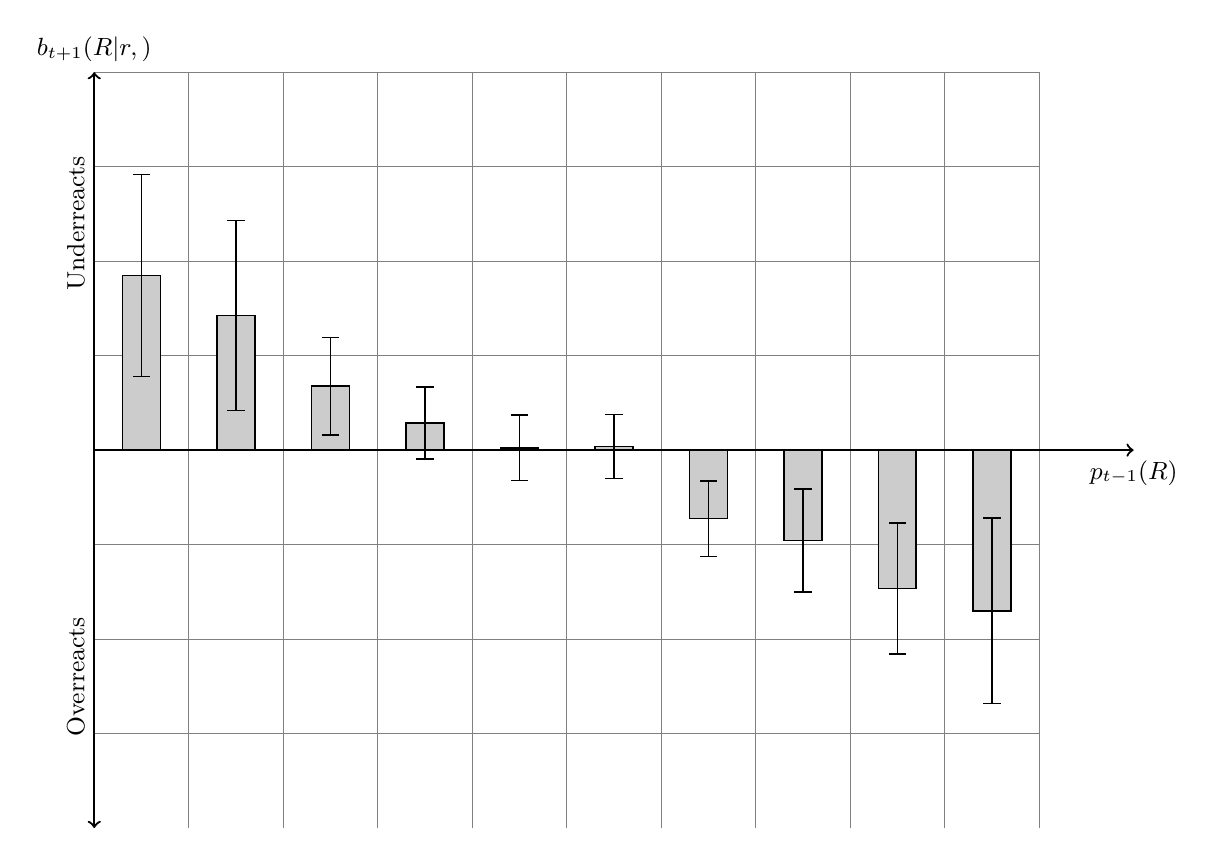
\begin{tikzpicture}[scale=12]
\draw[help lines,step=0.1] (0,-0.4) grid (1,0.4);
\filldraw[opaque,white!80!black] (0.03,0) rectangle (0.07,0.1847);
\draw[line width=0.6] (0.03,0) rectangle (0.07,0.1847);
\draw[line width=0.6,|-|] (0.05,0.0770) -- (0.05,0.2924);
\filldraw[opaque,white!80!black] (0.13,0) rectangle (0.17,0.1424);
\draw[line width=0.6] (0.13,0) rectangle (0.17,0.1424);
\draw[line width=0.6,|-|] (0.15,0.0410) -- (0.15,0.2438);
\filldraw[opaque,white!80!black] (0.23,0) rectangle (0.27,0.0675);
\draw[line width=0.6] (0.23,0) rectangle (0.27,0.0675);
\draw[line width=0.6,|-|] (0.25,0.0149) -- (0.25,0.1200);
\filldraw[opaque,white!80!black] (0.33,0) rectangle (0.37,0.0284);
\draw[line width=0.6] (0.33,0) rectangle (0.37,0.0284);
\draw[line width=0.6,|-|] (0.35,-0.0106) -- (0.35,0.0674);
\filldraw[opaque,white!80!black] (0.43,0) rectangle (0.47,0.0023);
\draw[line width=0.6] (0.43,0) rectangle (0.47,0.0023);
\draw[line width=0.6,|-|] (0.45,-0.0332) -- (0.45,0.0379);
\filldraw[opaque,white!80!black] (0.53,0) rectangle (0.57,0.0038);
\draw[line width=0.6] (0.53,0) rectangle (0.57,0.0038);
\draw[line width=0.6,|-|] (0.55,-0.0311) -- (0.55,0.0387);
\filldraw[opaque,white!80!black] (0.63,0) rectangle (0.67,-0.0725);
\draw[line width=0.6] (0.63,0) rectangle (0.67,-0.0725);
\draw[line width=0.6,|-|] (0.65,-0.1134) -- (0.65,-0.0317);
\filldraw[opaque,white!80!black] (0.73,0) rectangle (0.77,-0.0958);
\draw[line width=0.6] (0.73,0) rectangle (0.77,-0.0958);
\draw[line width=0.6,|-|] (0.75,-0.1514) -- (0.75,-0.0402);
\filldraw[opaque,white!80!black] (0.83,0) rectangle (0.87,-0.1466);
\draw[line width=0.6] (0.83,0) rectangle (0.87,-0.1466);
\draw[line width=0.6,|-|] (0.85,-0.2167) -- (0.85,-0.0765);
\filldraw[opaque,white!80!black] (0.93,0) rectangle (0.97,-0.1700);
\draw[line width=0.6] (0.93,0) rectangle (0.97,-0.1700);
\draw[line width=0.6,|-|] (0.95,-0.2691) -- (0.95,-0.0709);
\draw[line width=0.8,->]  (0,0) -- (1.1,0) node[below] {\small{$p_{t-1}(R)$}};
\draw[line width=0.8,<->] (0,-0.4) -- (0,0.4) node[above] {\small{$b_{t+1}(R|r,\xmark)$}};
\draw (0,0.24) node[above,rotate=90] {\small{Underreacts}};
\draw (0,-0.24) node[above,rotate=90] {\small{Overreacts}};
% ADD THEORY CURVE BELOW
\end{tikzpicture}
